\documentclass{article}

\usepackage{fancyhdr}
\usepackage[a4paper]{geometry}
\usepackage{enumerate}
\usepackage{xcolor}

\usepackage{graphicx}
\graphicspath{ {./} }

\setlength{\headheight}{15.2pt}
\pagestyle{fancy}
\lhead{Perl Programming Project}
\rhead{\'{A}lvaro Abella Bascar\'{a}n}

\newcommand{\spaces}{\space\space\space\space\space\space}
\newcommand{\g}[1]{\textcolor[rgb]{0,0.6,0}{#1}}
\newcommand{\re}[1]{\textcolor[rgb]{0.6,0,0}{#1}}
\newcommand{\bl}[1]{\textcolor[rgb]{0,0,0}{#1}}

\begin{document}

\title{Getting the Topmost Scoring Sequences from Position Weight Matrices
     \author{\'{A}lvaro Abella Bascar\'{a}n\\
     \texttt{alvaro.abella01@estudiant.upf.edu}}
     }
\maketitle

\newpage

%%%% PROBLEM DESCRIPTION %%%%
\section{Problem description} \label{problem}
\emph{
Position Weight Matrices are a simple way to model signals appearing on DNA and protein sequences. They summaryze the frequencies of every letter of the nucleotide or amino acid alphabets at a given position of the signal, for instance a splice site or a transcription factor binding site. This means that we can obtain a score, either from the absolute frequencies or by transforming them into log-likelihoods, for a given sequence to determine if it contains the signal pattern or not. Yet, they can also be used as sequence generators. The idea is to write a Perl script to produce all the possible sequences a PWM can match and report them ranked by score, for the shake of simplicity, we will work with nucleotides. On some cases, it can be unfeasible to produce all the possible sequences; the worst scenario is a PWM for a random sequence, where the score of any of the four nucleotides is 0.25, as the number of posible sequences will be 4n (being n the length of the matrix). For instance a matrix for a nucleotide signal made of 10 nucleotides, n=10, can generate 410 = 1048576 different sequences. As we do not want to fill the disk with too many sequences, we can set a cut-off, say here M=10000 sequences. However, we still must produce only the M sequences that have the highest scores. The simplest way to achieve that is to use a secondary PWM where the positions are reordered by the score of the most frequent nucleotide per position, as well as an array with the original positions, taken as scalar values, recording the order of the new PWM. The best approach can be a recursive function that start generating new sequences iterating over the nucleotides per position sorted from higher frequencies to lower ones. The output records should contain two fields, the generated sequence and the corresponding score, both can be calculated simultaneously. Finally, the script should read a text file containing the PWM in TRANSFAC format, having a section with five fields to store in memory (the ones marked in green, for the position and the relative frequencies for A, C, G and T, in that order). Below you can find two matrices that you have to run separately through your program. Discuss the results obtained from them on the report.
}

%%%% ALGORITHM %%%%
\section{Algorithm} \label{algorithm}
\subsection{Description} \label{alg:description}

After a first glampse to the problem it came obvious that, as we must produce only the sequences with highest scores and in an ordered way, the first step would be obtaining the highest scoring sequence. Once we have this sequence we can use it as the starting point to produce, by modification, new sequences in order of decreasing score. At this point our problem is subdivided in two subproblems: \emph{a) } How to produce the highest scoring sequence? and \emph{b) } How to obtain from it the \emph{n} sequences with highest score? Here is the solution I found:\\
\begin{enumerate}[a)]
\item In order to produce the highest scoring sequence I first ordered by decreasing score the elements at each position (row) of the PWM. Once this is done we can just take the first nucleotide at each position and we will obtain the highest scoring sequence. Of course, there can be more than one sequence with the same score, but any of them will be an equally good starting point for our algorithm. However, in order to have more reproducible results, I chose a stable sorting algorithm (just using the pragma \emph{ use sort `stable'}).

\item Producing from this sequence the \emph{n} highest-scoring sequences was a considerably more difficult problem. The first step to take was fairly easy: if we have the top-scoring sequence (from now on, \emph{sequence 1}), in order to obtain the second sequence we only have to modify the first one, applying the nucleotide change which decreases the score the least possible. After this we would have \emph{sequence 1} and its modified version \emph{sequence 2}.\\
\\
We now have a list of two sequences and ought to obtain the third one. We should iterate through each position of the two sequences and find the nucleotide change which produces the best possible scoring sequence different from the other two. We here encounter a problem, as we might find that the best change is the same as in the previous step, so that we would generate again the same sequence. To avoid this I decided to keep track of the changes applied to each sequence, such that if a given position of \emph{sequence 1} was modified to obtain \emph{sequence 2}, this position of \emph{sequence 1} is marked now as \emph{unmodifiable}, and will not be modified again.\\
\\
We have so far a working algorithm which starts with the highest scoring sequence and, at each step, produces the next top-scoring sequence, adding it to the list of top-scoring sequences. At each step all the sequences within this list will be analyzed to find the best nucleotide change, which will be applied to obtain the next sequence. There might be the case were there are several changes (say \emph{m} changes) which produce equally scoring sequences, and in this situation all this changes are considered and applied to obtain \emph{m} new sequences.\\
\\
During the course of the process it is probable that some sequence will be have been modified at all its positions, and thus should not be modified again. In order to speed up the algorithm, I thought of removing this sequence from the list of `modifiable top-scoring sequences', and storing it in another list. By this way we would avoid analyzing sequences which can't be modified. I found, however, that in this case we should at the end order all the sequences by score. After trying both approaches I decided to keep only one list, but skipping those sequence which are not modifiable, as this resulted to be faster and simpler.\\
\\
In order to produce only the \(n^{th}\) top-scoring sequences, we have to keep a count of how many sequences have been produced so far. Once the count has reached \emph{n}, the main loop of the algorithm breaks and we return the list of all sequences (umodifiable and modifiable sequences), which are already ordered by score.
\end{enumerate}

%%%% IMPLEMENTATION DETAILS %%%%
\subsection{Implementation details} \label{implementation}

As the program resulted to be a bit more complicated than I expected, I had to use quite a lot of encapsulation in order to make the program a bit more readable and easier to debug. The main part of the program is included in a module `PWM.pm'. This module contains a class responsible for loading the position weight matrix from a TRANSFAC-format file, storing it and producing the top-scoring sequences. In order to handle the sequences more easily I created another class called `Seq', which not only represents a sequence but also provides methods to obtain the length, calculate the score, etc., and among them the methods needed to know if a given position is modifiable or not. This two modules are stored in src/lib/.\\\\
The command line interface to the program is provided by the file /src/top\_scoring.pl. Below is the output of executing \emph{./top\_scoring.pl --help}:\\\\
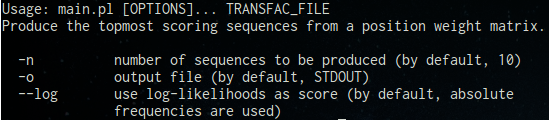
\includegraphics[scale=0.5]{perl}

\newpage

%%%% EFFICACY %%%%

\subsection{Efficiency of the algorithm} \label{efficiency}

There are two factors which affect the number of computations done by the algorithm. The first of them is the number of sequences desired by the user \emph{n}, and the second is the length of the sequences (\emph{l}), which is given by the number of rows of the Position Weight Matrix.\\
\\
The algorithm, as described in section \ref{algorithm}, is composed by an outer loop which iterates until \emph{n} sequences have been found. Inside this loop there is a loop which iterates over each sequence found so far (let's call \emph{ssf} to the number of sequences found so far, at a given moment), and inside this there is an even inner loop which iterates over each position of the sequence (1 to \emph{l}). Let us call a `cycle' to an iteration of the outermost loop. After a given cycle, we will have found in the best case \(l \cdot ssf\) possible changes (in other words, \(l \cdot ssf\) new sequences), and in the worst case, only 1 new sequence (if we find no new sequences, the algorithm would end).\\
\\
It is easy to see that, in the best case, after \emph{i} cycles we would have \(l^i\) sequences. In the worst case, however, we only find one sequence per cycle, and after \emph{i} cycles we will have \emph{i} sequences. If we want to obtain \emph{n} sequences, in the best case we will have:\\

\begin{equation} \label{eq:best_case_cycles}
  n_{seqs} = l^{num.cycles} \rightarrow num.cycles = \frac{log(n_{seqs})}{log(l)}
\end{equation}

Whereas in the worst case:

\begin{equation} \label{eq:worst_case_cycles}
  n.cycles = n_{seqs}
\end{equation}

However, we must take into account that there are two loops inside each cycle, one nested into the other, giving a total of \(ssf \cdot l\) iterations per cycle. If we consider the sum of all cycles, expressing \emph{ssf} as a function of the length \emph{l} and the number of cycles (equations \ref{eq:best_case_cycles} and \ref{eq:worst_case_cycles}), we get (after a short mathematical derivation which I am obviating), that in the best case:

\begin{equation} \label{eq:best_case_all_iters}
  n.iters = \frac{l^{
  					 2 + \frac{ln(n)}
  					 	 	  {ln(l)}}
  					 - l^2}
  			      {l-1} = \frac{n \cdot l^2 - l^3 - 1}
  			      			   {l - 1}
\end{equation}

And in the worst case:

\begin{equation} \label{eq:worst_case_all_iters}
  n.iters = \frac{l}{2} \cdot (n^2 + n)
\end{equation}

Finally, we have:\\
\\
Best case, with respect to \emph{l}:
\begin{equation}
\mathcal{O}(l)
\end{equation}
Best case, with respect to \emph{n}:
\begin{equation}
\mathcal{O}(n)
\end{equation}
Worst case, with respect to \emph{l}:
\begin{equation}
\mathcal{O}(l)
\end{equation}
Worst case, with respect to \emph{n}:
\begin{equation}
\mathcal{O}(n^2)
\end{equation}

\subsection{Utility of the program and possible upgrades} \label{upgrades}
Thinking about the uses of this program I concluded that a possible use would be to find in a very fast way those sequences which contain a given motif. If we have many sequences and want to check what ones contain a given motif with length \emph{m}, we would have to check the scores of each subsequence of length \emph{m} in each of the sequences. However this might be computationally costly, specially if the sequences are long. In this case, we could just use this program to produce the topmost scoring sequences, and then we would just have to make a search to find which of our sequences contain any of the topmost scoring sequences. As the topmost scoring sequences can be produced only once and then be reused, this might be a faster approach.\\
\\
If this program was to be used in this way, we might want to produce not the \emph{n} top scoring sequences, but all the sequences which have a score higher than a given threshold. This is an easy upgrade of the program, as it would involve just a modification of the main loop of the algorithm, which would stop not after \emph{n} sequences, but after finding a sequence with score below the given threshold.

\section{Results} \label{results}



\subsection{Motif 1}

In the first case we have a very simple matrix, with zeros at many positions. We can easily see that the highest scoring position must be \emph{GGACATGCCCGGGCATGTCC}, with only a tie in the last position, which can either be a \emph{C} or a \emph{T}. Running this program we should obtain that sequence as the first one (due to the stable sorting of each position), and the same sequence with \emph{T} at the last position as the second one. Running the program to produce only the first ten sequences gives us the following results (in green, the nucleotides which don't vary across the ten sequences, in red, nucleotides which vary in at least two sequences):\\\\
\emph{./top\_scoring.pl -n 10 motifs/motif1.tf}
\begin{center}
\re{GG}\g{ACATG}C\g{CCGGGCATGT}C\re{C}\spaces307\\
\re{GG}\g{ACATG}C\g{CCGGGCATGT}C\re{T}\spaces307\\
\re{GG}\g{ACATG}C\g{CCGGGCATGT}C\re{G}\spaces302\\
\re{GA}\g{ACATG}C\g{CCGGGCATGT}C\re{C}\spaces300\\
\re{GA}\g{ACATG}C\g{CCGGGCATGT}C\re{T}\spaces300\\
\re{GG}\g{ACATG}C\g{CCGGGCATGT}C\re{A}\spaces300\\
\re{AG}\g{ACATG}C\g{CCGGGCATGT}C\re{C}\spaces298\\
\re{GG}\g{ACATG}T\g{CCGGGCATGT}C\re{C}\spaces298\\
\re{GG}\g{ACATG}C\g{CCGGGCATGT}T\re{C}\spaces298\\
\re{AG}\g{ACATG}C\g{CCGGGCATGT}C\re{T}\spaces298\\
\end{center}

The results conform to our expectations. There are two sequences with the highest possible score (which match perfectly the consensus letters of the \emph{transfac} file), and we can see that the next sequences are mainly variations of the first ones in the last, second, and first positions. This is logical, as this positions are, in that order, the ones which show a smallest difference of frequency among the most frequent nucleotide and the second one. We can also see that the sequences are ordered by score. This is due to the algorithm, which produces only the top-scoring sequences in an ordered fashion (the sequences are not sorted at any moment).
\\
\subsection{Motif 2}
The results from the second motif are the following. In green, the nucleotides which don't vary. In red, those which vary in at least two sequences:\\\\
\emph{./top\_scoring.pl -n 10 motifs/motif2.tf}
\begin{center}

\re{ \g{AAT}T\g{TTCACGC}A\g{TGA}G\g{TT}\bl{C}\g{A}C } \spaces591\\
\re{ \g{AAT}T\g{TTCACGC}A\g{TGA}A\g{TT}\bl{C}\g{A}C } \spaces590\\
\re{ \g{AAT}C\g{TTCACGC}A\g{TGA}G\g{TT}\bl{C}\g{A}C } \spaces589\\
\re{ \g{AAT}T\g{TTCACGC}T\g{TGA}G\g{TT}\bl{C}\g{A}C } \spaces589\\
\re{ \g{AAT}T\g{TTCACGC}A\g{TGA}G\g{TT}\bl{C}\g{A}T } \spaces588\\
\re{ \g{AAT}C\g{TTCACGC}A\g{TGA}A\g{TT}\bl{C}\g{A}C } \spaces588\\
\re{ \g{AAT}T\g{TTCACGC}T\g{TGA}A\g{TT}\bl{C}\g{A}C } \spaces588\\
\re{ \g{AAT}T\g{TTCACGC}A\g{TGA}G\g{TT}\bl{A}\g{A}C } \spaces587\\
\re{ \g{AAT}T\g{TTCACGC}A\g{TGA}C\g{TT}\bl{C}\g{A}C } \spaces587\\
\re{ \g{AAT}T\g{TTCACGC}A\g{TGA}A\g{TT}\bl{C}\g{A}T } \spaces587\\

\end{center}

Again the results are logical: our sequences are correctly ordered and each sequence is a variation in one single nucleotide of one of the previous sequences. The positions in red vary more due to the fact that the difference among the most frequent nucleotide and the second most frequent in that position is smaller, which makes it easier to change it maintaining a hight score.

\end{document}
